\begin{exercise}{Expérience de Fizeau}{1}{Spé}
{Interference, trous d'Young}{lelay, centrale}

Soient deux trous d'Young distants de $a = 10$ mm, percés dans un écran opaque éclairé sous incidence normale par par une source ponctuelle $S$ monochromatique de longueur d'onde dans le vide $\lambda_0 = 585$ nm. $S$ est situé dans le plan médiateur des trous, au foyer principal d'une lentille convergente. On observe des phénomènes d'interférence sur un écran situé à $D = 20$ m des trous d'Young.

L'expérience de Fizeau consiste à placer devant chaque trou un tube horizontal de longueur $L = 5$ m rempli d'eau, les deux tubes étant traversés par la lumière sous incidence normale. On peut faire circuler dans ces tubes l'eau à $v_e = 7$ m/s dans des sens opposés.

\begin{figure}[H]
    \centering
    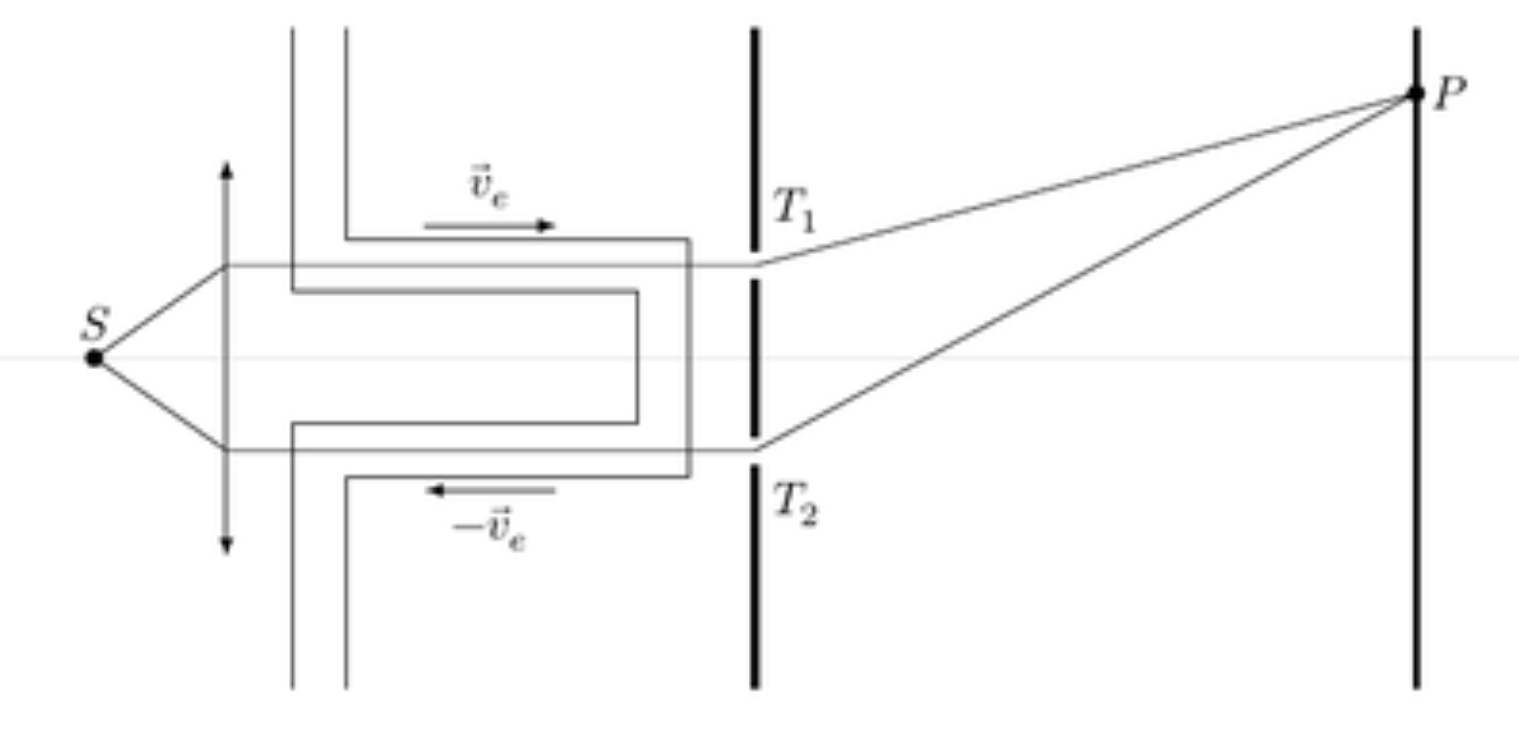
\includegraphics[width=.8\linewidth]{optique/interferences/expfizo.png}
    \caption{Schéma de l'expérience de Fizeau.}
\end{figure}

\begin{questions}
    \questioncours Différence de marche, ordre d'interférence
    \question Calculer l'ordre d'interférence au point $P$ en l'absence de courants d'eau ($v_e =0$).
    \uplevel{On suppose dans un premier temps que la vitesse de la lumière dans l'eau en mouvement à la vitesse $v_e$ vaut, dans le référentiel du laboratoire, $v = \frac{c_0}{n_e} + v_e$.}
    \question Justifier que cette hypothèse soit appelée `hypothèse galiléenne'.
    \question Calculer la variation de l'ordre d'interférence au point $P$ provoquée par l'établissement des courants d'eau.
    \question On observe un déplacement des franges de $\Delta x = 0.37 \pm 0.05$ mm, ceci est-il compatible avec l'hypothèse galiléenne ?
    \uplevel{On considère l'hypothèse relativiste suivante : la vitesse de la lumière dans l'eau en mouvement à la vitesse $v_e$ vaut, dans le référentiel du laboratoire, $v = \frac{c}{n_e} + v_e\qty(1-\frac1{n_e^2})$}
    \question Le déplacement des franges observé est-il en accord avec l'hypothèse relativiste ?
\end{questions}


\paragraph{Données :} Indice de l'eau au repos : $n_e = 1.337$

\end{exercise}